\subsection{\textit{Unified View of Parameter-Efficient Transfer Learning}}

\textit{Unified Parameter Transfer Learning} merupakan upaya untuk menggabungkan beberapa metode PEFT menjadi satu kesatuan \textit{framework} \parencite{uvpl}. Dalam \textit{transfer learning}, ide utamanya adalah mengambil \textit{pre-trained model} dan menyesuaikannya untuk tugas yang berbeda. Namun, ada banyak cara untuk melakukan adaptasi ini, dan setiap metode memiliki karakteristiknya masing-masing. Beberapa teknik mungkin fokus pada penambahan lapisan adaptasi, sementara yang lain mungkin memprioritaskan modifikasi parameter tertentu dalam model.

Metode PEFT lain telah berhasil mengubah atau menambahkan sedikit parameter untuk mendapatkan kinerja yang setara dengan \textit{fine-tuning} tradisional, tetapi hubungan antara metode tersebut tidak dimengerti secara baik \parencite{uvpl}. Selain itu, dicari juga elemen desain pada metode ini yang menjadi aspek penting pada kesuksesan metode terkait. \citeauthor{uvpl} pada penelitiannya ini, mencari hubungan antara tiap metode ini dengan mengupas arsitektur dari setiap metode terkait. Metode yang digunakan pada penelitian yang dilakukan oleh \citeauthor{uvpl} adalah LoRA, \textit{prefix-tuning}, dan \textit{adapter}.

\begin{figure}[ht]
    \centering
    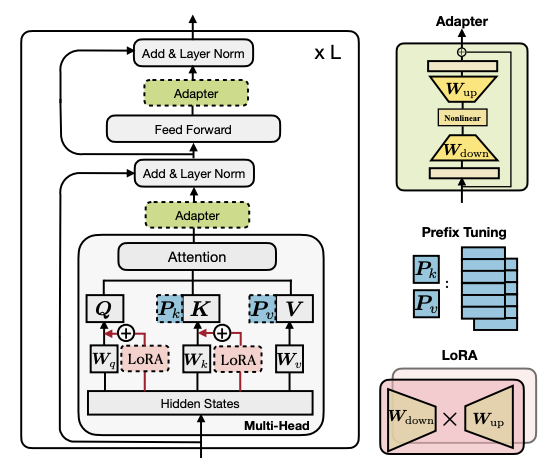
\includegraphics[width=0.8\textwidth]{chapter-2/uvpl.png}
    \caption{Arsitektur \textit{Unified View of Parameter-Efficient Transfer Learning} \parencite{uvpl}}
    \label{fig:uvpl}
\end{figure}

% TODO: tambahin secara jelas gimana tiap metode ini jadi satu dan hubungannya gimana
Arsitektur yang diajukan oleh \citeauthor{uvpl} pada penelitiannya dapat dilihat pada Gambar \ref{fig:uvpl}. Arsitektur tersebut menggabungan metode yang disebutkan sebelumnya pada model berbasis \textit{transformer}. 
